\section{Introduction} \label{sec:intro}
% P1 What is dysarthria? % Why is intelligilbity assessment important? 
Dysarthria is a motor speech disorder caused by weakness or paralysis of the articulators \cite{darley1972dysarthria}.
People with dysarthria often suffer from degraded speech intelligibility, repeated communication failures, and ultimately low quality of life. 
Accordingly, dysarthric speech assessments regarding speech intelligibility are conducted to check the patient's status and track the effectiveness of treatments \cite{kent1989toward}.
While the common way of dysarthric speech assessment is perceptual evaluation, the method is often subjective and laborious. 
Therefore, automatic speech assessment with objective and rapid results can assist clinicians in diagnosis and treatment planning.

%auxiliary diagnosis of clinical medicine

% To overcome such issues, research on the automatic assessment of dysarthric speech has been proposed, to assist clinicians' diagnoses and treatment planning with objective, reliable results.

% Hence, the automatic classification that highly correlates with the experts will have great potential for aiding clinicians in diagnosis and speech therapy.

% P2: Previous research 1
% Raw feature : Low Interpretability 
% Hand-crafted feature: Feature may be lossy
There are two main approaches to automatic assessment
of dysarthric speech. 
The first approach is to propose a list of hand-crafted features that are expected to capture the characteristics of dysarthric speech.
Explored feature sets include voice quality features \cite{narendra2021automatic}, prosody features \cite{hernandez2020prosody}, articulation or pronunciation features \cite{kim2012automatic, liu2021language}, and their combinations \cite{vasquez2018towards, yeo2022multilingual}.
This approach has the benefit of having medical implications, as it provides a transparent understanding of the features employed for automatic assessment. 
Nevertheless, this approach has the drawback that features that could be valuable in the assessment could be discarded during feature extraction.
The second approach involves leveraging the capabilities of neural networks (NNs), which can achieve better results by using raw inputs. \cite{yeo2022automatic, joshy2023dysarthria}.
% This method achieves better performance than the former method, with the benefit of allowing the model to self-learn the important features for the task. 
However, due to the black-box nature of NNs, the approach limits interpretability, which clinicians often crave for.

% karjigi2023speech
% P3: Previous 2
% Interpretable Neural Networks
 % Interpretability is important for clinical usage --> previous studies: CNN (sondes) 
\begin{figure}[t] %%% t: top, b: bottom, h: here
\centering
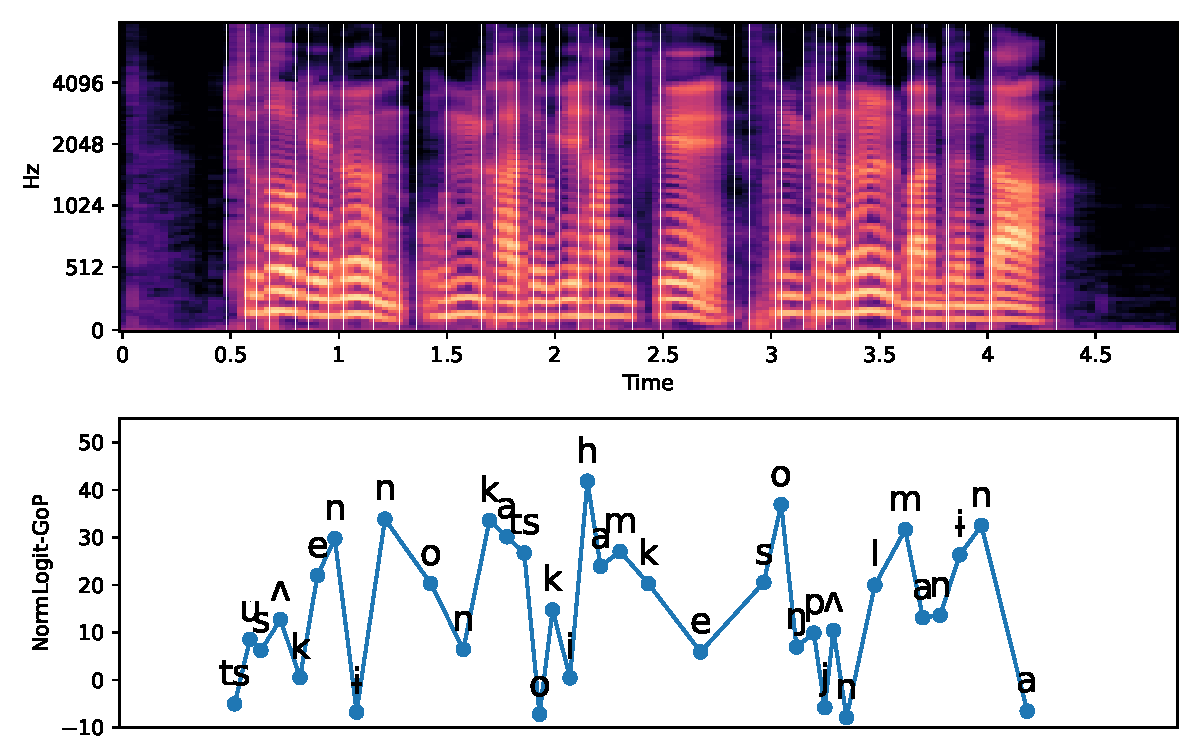
\includegraphics[width=0.97\columnwidth]{figures/fig_samplewise_gop.pdf}
\caption{
Example of GoP scores for each phone within an utterance.
Higher values indicate greater deviation from the correct pronunciation.
GoP scores allow easy identification of mispronounced phonemes.
}
\vspace{-1em}
\label{figs:samplewise_phones}
\end{figure}
Recent studies have attempted to integrate the benefits of both approaches, by enforcing the neural networks to learn the intermediate labels used for perceptual assessment, such as voice quality, articulation precision, nasality, and prosody \cite{tu2017interpretable, xu2021explore}.
Furthermore, certain studies focused on decoding misarticulation characteristics, which are the prominent aspect of dysarthric speech across languages \cite{yeo2022multilingual} and a significant factor that influences speech intelligibility \cite{de2002intelligibility}. 
For instance, the framework that measures the level of phonetic impairment was proposed by utilizing the activations of the hidden neuron \cite{abderrazek2022interpreting, abderrazek2022validation}.
While the method could provide overall phonetic characteristics of utterances, it is unable to provide assessments at the level of individual phonemes, which can help clinicians to pinpoint specific phonemes that require pronunciation training.

% which is essential for clinical applications such as pronunciation training.

% However, although the approach could offer information on averaged phonetic features of utterances, it did not provide phoneme-wise evaluations that are necessary to pinpoint specific phonemes that require improvement in clinical applications, such as pronunciation training. 

A common approach of phoneme-level speech assessment is to use the parallel NN that employs parallel datasets. 
The NN was trained using the same set of utterances recorded by both healthy speakers and patients to learn how to distinguish whether each phone in the utterances was from healthy or disordered speech \cite{miller2020assessing,quintas2022automatic}.
However, obtaining parallel datasets is a challenging task, especially for disordered speech.
Moreover, this approach often constrains the analysis to pre-defined speech materials, which may not capture the natural speech patterns utilized in everyday communication.

% For example, previous studies have utilized diadochokinetic exercises or pseudo-words as speech materials, which may not be representative of natural speech patterns.
% Furthermore, this limits the analysis to specific types of speech materials, which may not be representative of natural speech used in everyday communication, such as diadochokinetic exercises in \cite{miller2020assessing} and pseudo-words in \cite{quintas2022automatic}.


% P4: Misarticulation is the one of the major charactersitcs of dysarthria: Interpretability 를 개선하기 위해 GOP를 improve
% GOP + disordered speech
% GOP + wav2vec
\begin{figure*}[t!] % t: top, b: bottom, h: here
\centering
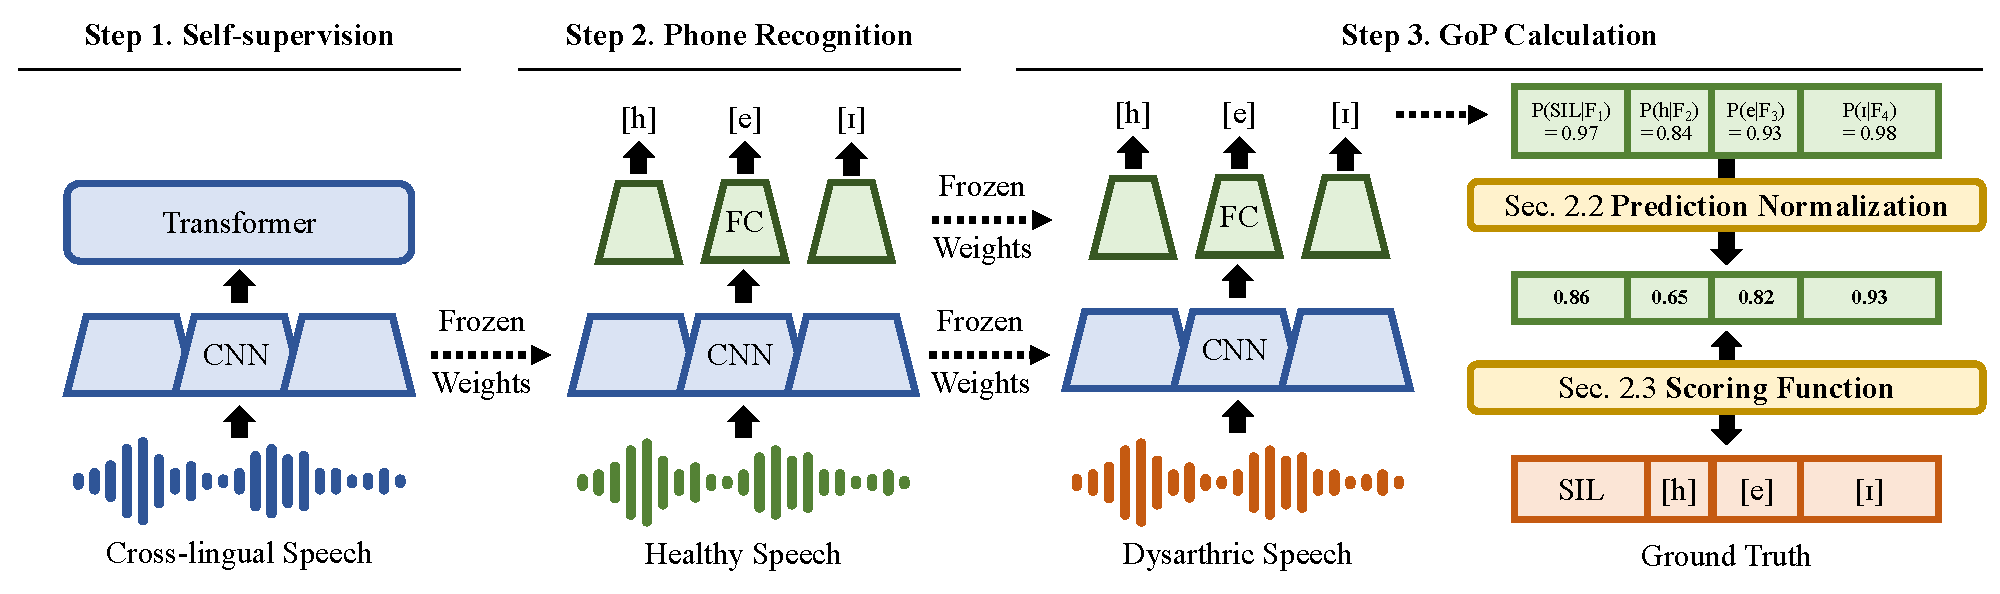
\includegraphics[width=1\textwidth,height=5cm]{figures/dysarthria-gop.pdf}
\caption{Overview of the improved GoP with UQ methods.}
\vspace{-1em}
\label{fig:diagram}
\end{figure*}

Another conventional approach of phoneme-level pronunciation evaluation is Goodness of Pronunciation (GoP) \cite{witt2000phone}.
GoP, which is defined as the degree of similarity between produced and correct pronunciation of phonemes, has two advantages in automatic speech assessments.
First, it provides detailed information on which phonemes are mispronounced and to what extent each phoneme is atypical.
Second, it does not necessitate a parallel dataset for model training.
% the approach eliminates the need for parallel recordings of healthy and atypical speech, making it a valuable tool for practical applications.
While GoP is often applied to non-native (L2) speech pronunciation assessment, some studies have also verified its potential use in assessing speech disorders as well \cite{pellegrini2014goodness,Fontan2015PredictingDS}.
% For example, the GoP-based assessment model correctly detected mispronounced phonemes from French-speaking unilateral facial palsy patients \cite{pellegrini2014goodness}. 
% Additionally, GoP showed strong correlations with comprehensibility ratings for diverse types of French-speaking patients \cite{Fontan2015PredictingDS}.


% Thus, to ensure optimal performance, it is crucial to consider the standardization of phone probabilities for GoP, as it relies heavily on acoustic model probabilities.
With the development of NNs, variants of GoP which employ probabilities from the state-of-the-art neural networks have been suggested \cite{hu2015improved,Cheng2020ASRFreePA,xu2021explore}.
However, using these probabilities without taking into account the modern NNs' tendency towards overconfidence can result in inaccurate conclusions:
NNs often generate probabilities close to $1.0$ even when their predictions are incorrect \cite{guo2017calibration}.
Since GoP relies heavily on probabilities, this can be especially problematic. The issue is compounded when the model encounters out-of-distribution (OOD) inputs, which are data that differ significantly from the training data's distribution \cite{hendrycks2017baseline}, such as dysarthric speech for healthy speech.
To alleviate such issues, UQ techniques, techniques to combat OOD problem \cite{guo2017calibration,hendrycks2017baseline}, can be applied.

% However, naive use of the probabilities from NN may lead to misleading conclusions due to the inherent overconfidence of modern NN.
% That is, NNs are often reported to output probabilities close to 1 even when their predictions are incorrect \cite{guo2017calibration}. 
% While this behavior can be critical to GoP as it heavily relies on probabilities, it becomes more problematic when the model encounters out-of-distribution (OOD) inputs, which refers to data that significantly differs from the distribution of the training data \cite{lee2018simple}. 
% To alleviate the issues, attempts to quantify uncertainty have been proposed, which is known as Uncertainty Quantification (UQ) methods. 

% Since GoP relies heavily on probabilities, this can be especially problematic. The issue is compounded when the model encounters out-of-distribution (OOD) inputs, which are data that differ significantly from the training data's distribution. To address these issues, researchers have proposed methods to quantify uncertainty, known as Uncertainty Quantification (UQ) methods.



% Dysarthric speech, like pathological speech, can be classified as OOD input since it differs greatly in acoustics from healthy speech. This paper proposes enhanced GoP variants for dysarthric speech evaluations by utilizing conventional Uncertain Quantification (UQ) techniques, which are known to tackle the OOD problem.

% directly applying methods from L2 assessment can result in suboptimal results. 
% In fact, a study on the analysis of L2 and disorder speech have shown different aspect \cite{}
% This issue becomes more problematic when the model encounters out-of-distribution (OOD) inputs, such as pathological speech that the model has not encountered during training \cite{lee2018simple}. 

This paper proposes improved GoP for automatic speech intelligibility assessment for dysarthric speech by employing Uncertainty Quantification (UQ) methods in two ways: (1) normalizing the phoneme prediction and (2) modifying the scoring function.
As pathological speech greatly differs in acoustics from healthy speech \cite{wilson2000acoustic}, dysarthric speech can be also understood as OOD input.
Therefore, we employ conventional UQ methods to improve GoP calculations for dysarthric speech assessment.
To assess the effectiveness of the improved GoP with UQ techniques, three dysarthric datasets, namely, UASpeech English, QoLT Korean, and SSNCE Tamil dataset, are utilized. 
To summarize, this paper redefines the current versions of GoP from a UQ standpoint and evaluates the effectiveness of UQ methods in improving GoPs.


% This paper aims to improve GoP for automatic speech intelligibility assessment of dysarthric speech, by regarding dysarthric speech as OOD samples for the NN.
% Hence, the Uncertainty Quantification (UQ) methods, which is a conventional technique to combat OOD problems, is applied on phoneme probabilities extracted from the fine-tuned Wav2Vec XLS-R model. 
% To check the efficacy of our improved GoP with UQ method, we use three dysarthric datasets, which include TORGO English, QoLT Korean, and SSNCE Tamil dataset.
% To sum up, this paper redefines the existing variants of GoP through the lens of UQ perspective, and verifies the efficacy of the conventional UQ methods for improved GoP.


% This paper presents improved GoP variants for automatic speech intelligibility assessment of dysarthric speech, by using Uncertainty Quantification (UQ) methods.
% UQ is a set of techniques used to estimate and understand uncertainty, and has been reported to show great performances in various domains.
% However, naive use of the NN may lead to misleading conclusions due to the inherent overconfidence of modern NN \cite{guo2017calibration}.
% That is, modern NNs often output probabilities close to 1, even when the network's predictions are incorrect.
% This issue becomes particularly problematic when the NN is presented with out-of-distribution (OOD) inputs, such as pathological speech, which the model has not seen during training \cite{lee2018simple}. 
% In fact, the vast acoustic difference of dysarthric speech from healthy speech have often impeded the technology applications developed for healthy speakers \cite{wilson2000acoustic}.

% Therefore, this paper considers pathological speech OOD input.


% This becomes especially problematic when NN has never seen the sample during training, often defined as out-of-distribution (OOD) inputs \cite{lee2018simple}.
% Considering its vast acoustic difference from healthy speech, pathological speech may be considered as OOD input. 
% Moreover, some studies reported \cite{}.
% Hence, directly applying methods from L2 assessment can result in suboptimal results \cite{wilson2000acoustic}.







% is known to help the model to combat miscalibration techniques. \cite{guo2017calibration,hendrycks2017baseline}.
% Therefore, 
% We revisit the existing variants of GoP through the lens of UQ and apply simple yet effective methods to improve upon them.



% However, predictions of modern neural networks have the tendency to produce uncalibrated and overconfident predictions \cite{guo2017calibration}.
% However, earlier investigations on GoP have neglected the significant intra-speaker and inter-speaker variability present in dysarthric speech. which can impede the application of other technologies on this type of speech \cite{wilson2000acoustic}. 



% , as it offers phoneme-level information without requiring parallel datasets.

% to combat its miscalibration.



% The rest of the paper is organized as follows: \Cref{sec:gop} introduces the improved GoPs by using the UQ methods. 
% \Cref{sec:experiment} describes the experiments, including datasets and details of our implementations for both baseline and proposed experiments.
% Results regarding the performances of the experiments and further analyses of essential phonemes for speech intelligiblity by languages are demonstrated in \Cref{sec:results}.
% Lastly, \Cref{sec:conclusion} is followed with a conclusion.

% by utilizing neural networks as a component inside the existing theoretical framework. 
% Some studies have sought to explain the neural network's decisions in terms of multiple dimensions such as vocal quality, articulation precision, nasality, and prosody \cite{tu2017interpretable, xu2023dysarthria}.
% While the approach can provide a comprehensive view of speech features, they cannot provide in-depth information for each aspect, which may have practical applications for clinical intervention. 

% The fundamental idea of applying GoP to disordered speech is to detect pathological phonemes that are different from that of healthy speech.

% Mispronounced phonemes can be identified using a threshold, which is often optimized using a validation set \cite{hu2015improved, xu2021explore}. 

% Hence, this paper utilizes GoP for automatic speech intelligibility assessment of dysarthric speech.


%%%again..
% This paper proposes an improved GoP for automatic speech intelligibility assessment of dysarthric speech, by using Uncertainty Quantification (UQ) methods.
% However, there are two drawbacks of existing GoP approaches, regarding the characteristics of dysarthric speech: (1) the scoring function is not expressive enough to capture uncertainty, and (2) the output phoneme prediction probabilities are uncalibrated.
% Hence, Uncertainty Quantification (UQ) methods are incorporated in GoP calculations, by (1) updating the scoring function and (2) modifying the phoneme predictor.
% UQ is a set of techniques used to estimate and understand uncertainty, and is known to help the model be more accurately calibrated, leading to more reliable predictions and better decision-making \cite{guo2017calibration,hendrycks2017baseline}. 
% To standardize the skewed phone probabilities, which is a notable characteristic of dysarthric speech, we anticipate that the inclusion of UQ will be beneficial for GoP calculations.
% To validate the effectiveness of our proposed method, three dysarthric datasets are tested, which includes  English, QoLT for Korean, and SSNCE for Tamil.

% This addresses two main shortcomings of existing GoP approaches, namely the insufficiently expressive scoring function and the uncalibrated phoneme prediction probabilities.
% UQ method is the technique have been proposed to correct bias in various research fields, such as computer vision and natural language processing (NLP) \needcite. 

% Hence, we improve GoPs by using UQ methods, which have been suggested to rectify bias in 

% In addition, to further reduce the language-specificness of the phoneme predictor, we leverage the recently introduced self-supervised model with cross-lingual training \cite{babu22_interspeech} to extract the speech features.


% The rest of the paper is organized as follows: \Cref{sec:gop} introduces the proposed approach of improving GoP by using the UQ methods. 
% \Cref{sec:experiment} describes the experiments, including the experimental setup of our implementations.
% Results regarding the performances of the experiments and further analyses of frequently mispronounced phones by languages are demonstrated in \Cref{sec:results}.
% Lastly, \Cref{sec:conclusion} is followed with a conclusion.


%Kaldi-based; GoP based: need largae amount of data for training


% Previous studies have leveraged the development of neural networks to propose variations of GoPs.
% Started from GMM-GoP \cite{witt2000phone}, studies proposed to calculate GoPs from Time-delayed neural network (NN-GoP) \cite{hu2015improved}, generative model \cite{Cheng2020ASRFreePA}, and Wav2Vec 2.0-based model \cite{xu2021explore}. 
% However, predictions of modern neural networks have the tendency to produce uncalibrated and overconfident predictions \cite{guo2017calibration}.
% That is, even when the network's predictions are incorrect, the model often outputs probabilities close to 1.
% % This greatly degrades the trustworthiness and reliability of neural networks. 
% Considering GoP is highly dependent on the probabilities of the neural networks, such bias can greatly hinder the performance of GoPs. 
% To address these concerns, uncertainty quantification (UQ) techniques have been suggested to rectify bias in various research fields such as computer vision and natural language processing (NLP) \needcite.
% Therefore, this paper incorporates UQ methods in the speech domain, particularly, in GoP score calculations for dysarthric speech assessments.

% Given the numerous advancements of UQ methods, the natural progression of it is to apply them to GoP.

% especially for tasks such as confidence calibration and out-of-distribution (OOD) detection.
% Confidence calibration aims to match the prediction probabilities to represent the true correctness likelihood \cite{guo2017calibration}, and OOD detection tries to detect the samples that are highly different from the training samples \cite{lee2018simple}.

% P5: Propose model
% Phone-level assessment method of dysarthric speech
% Focus on improving the well-known examination of phone-level assessments: Goodness of Pronunciation (GOP)
% we suggest a novel way of understanding the GOP predictions with the lens of out-of-distribution detection, where numerous advances have been made on OOD in the past decade.
% other ood methods도 활용해서 보여주겠다
% we further leverage the power of cross-lingual self-supervision to avoid the language bias inherent inside the acoustic models of GOP




% and \Cref{sec:discussion} further demonstrates analyses of frequently mispronounced phones by severity levels and languages detected by our best-performing method. Lastly, \Cref{sec:conclusion} is followed with a conclusion.

%performance of proposed models is evaluated with existing mainstream methods

% for classification. \Cref{sec:speech_corpus} presents three datasets: TORGO for English, QoLT database for Korean, and SSNCE database for Tamil. Finally, \Cref{sec:setup} describes the experimental settings and reports classification results, which is followed by a conclusion in \Cref{sec:dis_con}.

% Contribution
%% Detailed Assessment Results with phone-level assessment
% 기존 GOP를 OOD로 재해석해서 성공적으로 잘활용되고 있는 OOD의 literature를 사용.
% Rethinking of 

% ------------

% P5 Propose model
% SSL representations + OOD 사용



% asr-dependency
% prob 1: asr 성능을 높이려면: ctc/rnn-t -> acoustic model만 있는게 아니고, language model 능력도 transformer에다가 밀어넣음. (food: fud -> fo[sep]od -> "food"라는 단어를 이해 -> 앞뒤를 보고 넣은거 -> receptive field가 전체를 보고 있음 vs. phoneme recognition (local하게 phone 제대로 발음했니?)
% -> target: phone (ipa) -> inherently introduces language independence
% prob 2: softmax() -> inherently dependent on other phone class prob. -> [0.5, 0.5] = (1) 둘다 probable하다 (2) 둘다 improbable하다
%   

% One aspect is to explain articulatory or pronunciation characteristics  
% For exmplae, studies have focused on analyzing articulation or pronunciation, which plays a significant role in speech intelligibility \cite{de2002intelligibility}. 

%--------------------------------------------
% consonant-vowel transition, 
% For example, a jointly trained fully-connected neural network with a severity label at the output layer and four perceptual labels (nasality, vocal quality, articulatory precision, prosody) at the intermediate layer was proposed \cite{tu2017interpretable}.
% The model demonstrated better accuracy and interpretability, by explaining the final decisions with a set of explanatory features, which include nasality, vocal quality, articulatory precision, and prosody. 
% Another study trained the CNN-based model to jointly learn a classification label and four clinically-interpretable features, by adding an interpretable layer after the output layer.
% Interpretable layer consisted of four units, each learning the acoustic aspects of articulation precision, consonant-vowel transition precision, hypernasality, and vocal quality \cite{xu2023dysarthria}.
% In addition, Shapley additive explanation (SHAP) was applied to further analyze the contribution of each acoustic feature in the interpretable layer to the final prediction.
% The interpretable layer consisting of 4 units are trained to learn the acoustic features that characterizes different aspects of dysarthria interpretable to clinicians.

%-------------------------------------------
% Previous studies includes Neuro-based Concept Detector \cite{abderrazek2022interpreting, abderrazek2022validation}, 

% On the other hand, some studies focused on the analysis into misarticulation, which is the prominent characteristic of dysarthric speech across languages \cite{yeo2022multilingual}.
% Neuro-based Concept Detector was demonstrated to reflect the level of impairment of the phonetic features through its hidden neurons' activation patterns \cite{abderrazek2022validation,abderrazek2022interpreting}.
% Features using phonological posterior probabilites obtained by parallel bi-directional recurrent neural networks were used to determine the severity level of dysarthria \cite{miller2020assessing}.
% The automatic prediction model based on a siamese network that computes similarity scores between healthy and pathological consonants were proposed \cite{quintas2022automatic}.
% This study also aims to investigate the incorrectly pronounced phonemes and utilize this information for automatic speech intelligibility assessment of dysarthric speech.

 % to promote interpretability in terms of the pronunciation of the consonants 
%comprehensive %auxiliary diagnosis of clinical medcine

% An objective articulation measure of the consonant-vowel transitions was derived based on the posteriors of a convolutional neural network \cite{mathad2022consonant}.



% Some studies have sought to explain the neural network's decisions in terms of multiple dimensions such as vocal quality, articulation precision, nasality, and prosody \cite{tu2017interpretable, xu2023dysarthria}.
% While the approach can provide a comprehensive view of speech features, they cannot provide in-depth information for each aspect, which may have practical applications for clinical intervention. 

% Other studies concentrated on the analysis of phoneme-level pronunciation \cite{miller2020assessing,quintas2022automatic}.
% Although such models may not generate extensive interpretable insights provided by previously-mentioned studies, they have an advantage in offering information on what phonetic features or phonemes are atypical.

% Therefore, this study adopts the second approach, and examines mispronounced phonemes and utilizes the information for automatic speech intelligibility assessment of dysarthric speech.

% a prominent characteristic of dysarthric speech across languages \cite{yeo2022multilingual}, and 

% Another approach is to analyze the activation patterns of the hidden neurons associated with phonetic features 

% With such advantages, GoP has been utilized to automatically assess atypical speech, including non-native speech \cite{} and disordered speech \cite{}.

% Variations of GoP have leveraged the development of neural networks. 
% While GMM-GoP was the starting point \cite{witt2000phone}, subsequent studies proposed calculating GoPs from Time-delayed neural networks (NN-GoP) \cite{hu2015improved}, generative models \cite{Cheng2020ASRFreePA}, and Wav2Vec 2.0-based models \cite{xu2021explore}. 
% However, modern neural networks tend to generate uncalibrated and overly confident predictions. 
% That is, even when they are incorrect, leading to probabilities close to 1 \cite{guo2017calibration}. 
% Since GoP heavily depends on the neural networks' probabilities, such biases can significantly impede the performance of GoPs. 
% To address these concerns, uncertainty quantification (UQ) techniques have been proposed to correct bias in various research fields, such as computer vision and natural language processing (NLP) \needcite. 
% Therefore, this paper introduces UQ methods in the speech domain, particularly in GoP calculations.

% To overcome these issues, this paper employs Goodness of Pronunciation (GoP) for automatic speech intelligibility assessment in dysarthric speech. 
% Goodness of Pronunciation (GoP) is the metric that scores pronunciation of atypical speech at a phoneme level.
% GoP uses the posterior probability of the correct phone, obtained from acoustic models, along with the speech segment of the corresponding phone \cite{witt2000phone}. 

% However, parallel networks often require parallel datasets in training the models to recognize and differentiate between various phonemes or speech sounds due to the difficulty in obtaining parallel datasets. 
% obtaining these parallel datasets can be particularly challenging for disordered speech datasets, which makes it difficult to obtain matched speech samples between individuals with speech disorders and healthy speakers.
% Despite the promising results, parallel networks often require parallel datasets to train the models to recognize and distinguish between different phonemes or speech sounds, which is often difficult to be obtained for disordered speech dataset.
% Without parallel datasets, it can be challenging to train the network to differentiate between the target phonemes and other sounds that may be present in the speech signal.
% , which is challenging for disordered speech corpus. 

% Likewise, parallel networks often require parallel datasets, to train the models to recognize and distinguish between different phonemes or speech sounds.
% This limits the applications in a clinical setting, as it is difficult to obtain parallel datasets.
% One of the major limitations of parallel networks is that they often require parallel datasets to train the models to effectively recognize and differentiate between various phonemes or speech sounds. 

% However, the research was limited to diadochokinetic exercises. 
% Again, the study constrains the materials to 52 pseudo-words.

% However, this study was also limited in that it used only 52 pseudo-words as materials.

% This can pose a challenge in a clinical setting, particularly for disordered speech datasets, as obtaining appropriate parallel datasets can be difficult due to the idiosyncratic speech patterns and individual differences in speech production. Therefore, while parallel networks have shown potential for phoneme-level assessments, the need for parallel datasets can limit their applications in clinical settings.


% For instance, parallel bi-directional recurrent neural networks were presented to extract phonological posterior probabilities to assess the severity level of dysarthria \cite{miller2020assessing}.
% % Another study proposed the use of a siamese network to compute similarity scores between healthy and pathological consonants, in order to predict intelligibility scores for Head and Neck Cancer speech \cite{quintas2022automatic}.
% However, parallel networks often require parallel datasets to train the models to effectively recognize and differentiate between various phonemes or speech sounds.